% SETUP
\documentclass[11pt]{article}
\linespread{1.1}
\usepackage[utf8]{inputenc}
\usepackage{graphicx, amsmath, array, graphics, amssymb, epsfig, psfrag, geometry, alltt, subfiles, blindtext, pdfpages, mathtools, float}
\usepackage[export]{adjustbox}
\usepackage{fancyhdr}
\usepackage{array}
\usepackage{hyperref}

%%%%%%%%%%%%%%  code listing
\usepackage{listings}
\usepackage{color} %red, green, blue, yellow, cyan, magenta, black, white
\definecolor{mygreen}{RGB}{2,94,33} % color values Red, Green, Blue
\definecolor{mylilas}{RGB}{170,55,241}

\lstset{language=Matlab,%
    %basicstyle=\color{red},
    breaklines=true,%
    morekeywords={matlab2tikz},
    keywordstyle=\color{blue},%
    morekeywords=[2]{1}, keywordstyle=[2]{\color{black}},
    identifierstyle=\color{black},%
    stringstyle=\color{mylilas},
    commentstyle=\color{mygreen},%
    showstringspaces=false,%without this there will be a symbol in the places where there is a space
    numbers=left,%
    numberstyle={\tiny \color{black}},% size of the numbers
    numbersep=9pt, % this defines how far the numbers are from the text
    emph=[1]{for,end,break},emphstyle=[1]\color{black}, %some words to emphasise
    %emph=[2]{word1,word2}, emphstyle=[2]{style},    
}

\geometry{a4paper, top = 20mm, bottom = 20mm, left = 15mm, right = 15mm}
\DeclarePairedDelimiter\set\{\}

% Headers
\pagestyle{fancy}
\fancyhf{}
\chead{ELEN90064 Advanced Control Systems - Workshop 3 Report}
\cfoot{\thepage}

\begin{document}
% Cover Sheet

\includepdf{EngCSW3_1.pdf}
\clearpage
\setcounter{page}{1}

% Title
\begin{center}
\textbf{\Large{Emulation and Discrete Time Design}}\\
Group 56: Josh Foleti [639409], Liam Traynor [694783], YiLin Inez Zheng [702279], \\
Workshop: Friday 1:00pm - 3:00pm Luis, Due: 13/09/19  
\end{center}

%%%%%%%%%%%%% BEGIN INTRODUCTION %%%%%%%%%%%%%%%%%
\section{Introduction}
The aim of this workshop is to investigate the effects of sampling time from discretisation via different emulation methods. The PID controller from Workshop 2 will be discretised to stabilise the Quanser Aero at a pitch angle of $10^{\circ}$. The continuous plant from Workshop 2 will also be discretised and the aim is to achieve the same outcome by designing a discrete PI controller.   

% Some description about what we did, steps for analysis and design
\subsection{Method}
\begin{enumerate}
    \item %1
    Theoretically derive the discrete transfer functions for the PID controller $C(s)$ from Workshop 2 using the emulation approach:
    \begin{enumerate}
        \item %a
        $C_1(z)$ - Simple Approach
        \item %b
        $C_2(z)$ - Using Step Invariant/Zero-Order-Hold (ZOH)
        \item %c
        $C_3(z)$ - Bilinear Transformation with Pre-warping
    \end{enumerate}
    \item %2
    Simulate each $C(z)$ approach to find a sampling time $\Delta$ for when the closed loop system begins to become unstable. Test and record this on the Quanser Aero.
    \item %3
    Theoretically derive an expression $G(z)$ for the discrete transfer function for the 1DOF plant $G(s)$ from Workshop 2. Use a chosen emulation method and the respective sampling period $\Delta$ from the tested results.
    \item %4
    Design and simulate a discrete PI controller to stabilise the system at $10^{\circ}$. 
    \item %5
    Implement the PI controller and tune it on the Quanser Aero.
\end{enumerate}

%%%%%%%%%%%% BEGIN CALCULATION SECTION %%%%%%%%%%%%%%%%
\section{Discretisation Calculations}\label{section:calcs}
From Workshop 2, the final tuned PID controller $C(s)$ is in Eq.\ref{eq:Cs} and the Quanser Aero 1DOF transfer function with  experimental parameters is in Eq.\ref{eq:Gs}, 
\begin{equation}\label{eq:Cs}
    C(s) = k_p + \frac{k_i}{s} + k_d s = 3.6364 + \frac{3.5874}{s} + 3.271s
\end{equation}
\begin{equation}\label{eq:Gs}
    G(s) = \frac{\frac{K_t D_t}{J_p}}{s^2 + \frac{-b_p}{J_p}s + \frac{M_b g D_m}{J_p}} = \frac{0.06994}{s^2 + 0.1724s + 3.819}
\end{equation}
\subsection{Discretising C(s) to C(z) using three different methods of Emulation}
% Cs to Cz
\subsubsection{Emulation using Simple Approach}
% Simple apprach Cz1
The simple approach uses direct substitution of variables converting from Laplace domain to Delta domain and to Shift (z) domain. The variables are substituted such that $C(z) = C(\gamma)|_{\gamma = \frac{z - 1}{\Delta}}$ and $C(\gamma) = C(s)|_{s = \gamma}$.
\begin{align*}
    C_A(\gamma) &= C(s)|_{s = \gamma} = k_p + \frac{k_i}{\gamma} + k_d \gamma\\
    C_A(z) &= C_1(\gamma)|_{\gamma = \frac{z-1}{\Delta} } = k_p + \frac{k_i}{\frac{z-1}{\Delta}} + k_d \frac{z-1}{\Delta}
\end{align*}
\begin{equation}\label{eq:CAz}
    C_A(z)= \frac{\frac{k_d}{\Delta} z^2 + (k_p - \frac{2 k_d}{\Delta})z + (- k_p + k_i \Delta + \frac{k_d}{\Delta})}{z-1}
\end{equation}
\subsubsection{Emulation using Step Invariant Method (ZOH)}
% ZOH Cz2
This method generates the discrete controller with zero order hold samples. In general the results from this emulation method will match the time domain step response of the system more closely.
\begin{align*}
    C_B(z) &= (1 - z^{-1}) \mathcal{Z} \set[\Bigg]{ \mathcal{L}^{-1} \set[\Bigg]{\frac{C(s)}{s} } \Biggr|_{t=k\Delta} }\\
    &= (1 - z^{-1}) \mathcal{Z} \set[\Bigg]{ \mathcal{L}^{-1} \set[\Bigg]{\frac{k_p}{s} + \frac{k_i}{s^2} + k_d} \Biggr|_{t=k\Delta} }\\
    &= (1 - z^{-1}) \mathcal{Z} \set[\big]{ ( k_p u(t) + k_i t u(t) + k_d \delta (t) )   |_{t=k\Delta}}\\
    &= (1 - z^{-1}) \Biggr( \frac{k_p}{1 - z^{-1}} + \frac{\Delta k_i z^{-1}}{(1 - z^{-1})^2} + k_d \Biggr)\\
    &= k_p + \frac{\Delta k_i z^{-1}}{1 - z^{-1}} + k_d (1 - z^{-1})\\
    &= \frac{(k_p + k_d) + (-k_p + \Delta k_i - 2 k_d)z^{-1} + k_d z^{-2}}{1 - z^{-1}}
\end{align*}
\begin{equation}\label{eq:CBz}
    C_B(z)= \frac{(k_p + k_d)z^2 + (-k_p + \Delta k_i - 2 k_d)z + k_d}{z^2 - z}
\end{equation}
\subsubsection{Emulation using Bilinear Transform with Pre-warping}
% Bilinear Cz3
Similar to the simple approach, the transfer functions are transformed through the Laplace domain, Delta domain and Shift (z) domain. Here, a variable $\alpha$ is introduced, which is a Bode diagram reading of the peak frequency after the natural frequency drop in the close loop sensitivity function $S = \frac{1}{1 + CG}$. Therefore, $C(z) = C(\gamma)|_{\gamma = \frac{z - 1}{\Delta}}$ and $C(\gamma) = C(s)|_{s = \frac{\alpha \gamma}{\frac{\Delta}{2} \gamma + 1}}$.
\begin{align*}
    C_C(\gamma) &= C(s)|_{s = \frac{\alpha \gamma}{\frac{\Delta}{2} \gamma + 1}} = k_p + \frac{k_i}{\frac{\alpha \gamma}{\frac{\Delta}{2} \gamma + 1}} + k_d \frac{\alpha \gamma}{\frac{\Delta}{2} \gamma + 1}\\
    &= k_p + \frac{k_i \bigg( \frac{\Delta}{2} \gamma + 1 \bigg)}{\alpha \gamma} + k_d \frac{\alpha \gamma}{\frac{\Delta}{2} \gamma + 1}\\
    C_C(z) &= C_3(\gamma)|_{\gamma = \frac{z-1}{\Delta} }\\
    &= k_p + \frac{k_i \bigg( \frac{\Delta}{2} \frac{z-1}{\Delta} + 1 \bigg)}{\alpha \frac{z-1}{\Delta}} + k_d \frac{\alpha \frac{z-1}{\Delta}}{\frac{\Delta}{2} \frac{z-1}{\Delta} + 1}\\
    &= k_p + \frac{k_i \Delta (z -1 + 2)}{2 \alpha (z-1)} + \frac{k_d 2 \alpha (z-1)}{\Delta (z-1+2)}\\
    &= \frac{k_p [2\alpha \Delta (z-1)(z+1)] + k_i[{\Delta}^2 (z+1)^2] + k_d [4{\alpha}^2 (z-1)^2]}{2\alpha \Delta (z-1)(z+1)}
\end{align*}
\begin{equation}\label{eq:CCz}
    C_C(z)= \frac{(k_p + \frac{k_i \Delta}{2 \alpha} + \frac{k_d 2 \alpha}{\Delta})z^2 + (\frac{k_i \Delta}{\alpha} + \frac{k_d 4 \alpha}{\Delta})z + (-k_p + \frac{k_i \Delta}{2 \alpha} + \frac{k_d 2 \alpha}{\Delta})}{z^2-1}
\end{equation}
\subsection{Discretising G(s) to G(z) using three different methods of Emulation}
% Gs to Gz
Using the same three methods of emulation for the controller we discretise the linearised plant model $G(s)$. To make expression tidier, we used the coefficients $a_0=3.819$,$a_1=0.1724$ and $b_0=0.06994$ instead of the raw numeric values. This is shown in Eq.\ref{eq:Gs1} below,
\begin{equation}\label{eq:Gs1}
    G(s) = \frac{0.06994}{s^2 + 0.1724s + 3.819} = \frac{b_0}{s^2 + a_1 s + a_0}
\end{equation}
\subsubsection{Emulation using Simple Approach}
Similar to converting the controller, direct substitution was used for the variables $G(z) = G(\gamma)|_{\gamma = \frac{z - 1}{\Delta}}$ and $G(\gamma) = G(s)|_{s = \gamma}$.
\begin{align*}
    G_A(\gamma) &= G(s)|_{s = \gamma} = \frac{b_0}{\gamma^2 + a_1 \gamma + a_0}\\
    G_A(z) &= G_A(\gamma)|_{\gamma = \frac{z-1}{\Delta} } = \frac{b_0}{\big(\frac{z-1}{\Delta}\big)^2 + a_1 \frac{z-1}{\Delta} + a_0}
\end{align*}
\begin{equation}\label{eq:GAz}
    G_A(z)= \frac{b_0 \Delta^2}{z^2 + (a_1 \Delta -2)z + (1 - a_1 \Delta + a_0 \Delta^2)}
\end{equation}
\subsubsection{Emulation using Step Invariant Method (ZOH)}
This method proved quite complex due to the z-transform of 
\begin{align*}
    G_B(z) &= (1 - z^{-1}) \mathcal{Z} \set[\Bigg]{ \mathcal{L}^{-1} \set[\Bigg]{\frac{G(s)}{s}} \Biggr|_{t=k\Delta} }\\
    &= (1 - z^{-1}) \mathcal{Z} \set[\Bigg]{ \mathcal{L}^{-1} \set[\Bigg]{\frac{b_0}{s^3 + a_1 s^2 + a_0 s}} \Biggr|_{t=k\Delta} }\\
    &= (1 - z^{-1}) \mathcal{Z} \set[\Bigg]{ \mathcal{L}^{-1} \set[\Bigg]{\frac{b_0}{a_0}\cdot\frac{1}{s} + \frac{b_0}{a_0}\cdot\frac{s + a_1}{(s+a_1)^2 + (-a_1^2 + a_0)}} \Biggr|_{t=k\Delta} }\\
    &= (1 - z^{-1}) \mathcal{Z} \set[\big]{ ( \frac{b_0}{a_0}u(t) + \frac{b_0}{a_0} e^{-a_1 t}\cos((a_0 - a_1)^2 t)u(t) ) |_{t=k\Delta} }\\
    &= (1 - z^{-1}) \Biggr(\frac{b_0}{a_0}\cdot\frac{1}{1-z^{-1}} + \frac{b_0}{a_0}\cdot\frac{1 - e^{-a_1 \Delta}z^{-1}\cos((a_0 - a_1^2)\Delta)}{1 - 2e^{-a_1 \Delta}z^{-1}\cos((a_0 - a_1^2)\Delta) + e^{-2a_1 \Delta}z^{-2}} \Biggr)\\
    &= \frac{b_0}{a_0} \Biggr( 1 + \frac{(1 - z^{-1})\big(1 - e^{-a_1 \Delta}z^{-1}\cos((a_0 - a_1^2)\Delta)\big)}{1 - 2e^{-a_1 \Delta}z^{-1}\cos((a_0 - a_1^2)\Delta) + e^{-2a_1 \Delta}z^{-2}} \Biggr)\\
    &= \frac{b_0}{a_0} \Biggr(\frac{2 - \big(3e^{-a_1 \Delta}\cos((a_0 - a_1^2)\Delta) + 1 \big)z^{-1} + \big(e^{-2a_1 \Delta} + e^{-a_1 \Delta}\cos((a_0 - a_1^2)\Delta)\big)z^{-2}}{1 - 2e^{-a_1 \Delta}\cos((a_0 - a_1^2)\Delta)z^{-1} + e^{-2a_1 \Delta}z^{-2}} \Biggr)
\end{align*}
\begin{equation}\label{eq:GBz}
    G_B(z)= \frac{b_0}{a_0} \Biggr(\frac{2z^2 - \big(3e^{-a_1 \Delta}\cos((a_0 - a_1^2)\Delta) + 1 \big)z + \big(e^{-2a_1 \Delta} + e^{-a_1 \Delta}\cos((a_0 - a_1^2)\Delta)\big)}{z^2 - 2e^{-a_1 \Delta}\cos((a_0 - a_1^2)\Delta)z + e^{-2a_1 \Delta}} \Biggr)
\end{equation}
\subsubsection{Emulation using Bilinear Transform with Pre-warping}
Using the same value of $\alpha$ as when discretising $C(s)$, variable substitutions are made such that $G(z) = G(\gamma)|_{\gamma = \frac{z - 1}{\Delta}}$ and $G(\gamma) = G(s)|_{s = \frac{\alpha \gamma}{\frac{\Delta}{2} \gamma + 1}}$.
\begin{align*}
    G_C(\gamma) &= G(s)|_{s = \frac{\alpha \gamma}{\frac{\Delta}{2} \gamma + 1}} = \frac{b_0}{\big(\frac{\alpha \gamma}{\frac{\Delta}{2} \gamma + 1}\big)^2 + a_1 \frac{\alpha \gamma}{\frac{\Delta}{2} \gamma + 1} + a_0}\\
    &= \frac{b_0(\frac{\Delta}{2} \gamma + 1)^2}{(\alpha \gamma)^2 + a_1 \alpha \gamma(\frac{\Delta}{2} \gamma + 1) + a_0(\frac{\Delta}{2} \gamma + 1)^2}\\
    G_C(z) &= G_C(\gamma)|_{\gamma = \frac{z-1}{\Delta} } = \frac{b_0(\frac{\Delta}{2} \frac{z-1}{\Delta} + 1)^2}{(\alpha \frac{z-1}{\Delta})^2 + a_1 \alpha \frac{z-1}{\Delta}(\frac{\Delta}{2} \frac{z-1}{\Delta} + 1) + a_0(\frac{\Delta}{2} \frac{z-1}{\Delta} + 1)^2}
\end{align*}
\begin{equation}\label{eq:GCz}
    G_C(z) = \frac{b_0 \Delta^2 (z+1)^2}{(2\alpha(z-1))^2 + 2a_1 \alpha \Delta (z-1)(z+1) + a_0 \Delta^2 (z+1)^2}
\end{equation}

%%%% BEGIN SIMULATION SECTION %%%%
\section{Simulation and Experimental Testing of Sampling Periods}\label{section:sims}
%From Section \ref{section:calcs}, we implemented the discretized plants $C_A(z)$, $C_B(z)$ and $C_C(z)$ in Simulink and ran simulations across several sampling periods to establish where the system became unstable. Similar times were tested on the Quanser Aero to obtain experimental data for comparison and analysis.\\ - not sure if this is necessary... 

The same PID gains from Workshop 2 were plugged in to Simulink blocks for simulating and experimentally testing the discretised controllers ($k_p = 50.9091$, $k_i = 50.2242$, $k_d = 45.7893$). A minor adaptation was made to express the $k_d z$ term in the controller $C(z)$ as $k_d \frac{N}{1 + N\Delta \frac{1}{z-1}}$, where $N$ was set to an arbitrary 20, in order to make $C(z)$ proper.\\

In the Quanser Aero Simulink model, the gain block following the controller was set to $1$ in order for the PID gains to act directly on the system. After trialling, it was found that a gain of $0.5$ gave responses that matched the simulation results better due to the split output voltage for two motors. %uh... not too sure if this is right...

\subsection{Simple Approach Discrete Controller}
% So I'm not sure if we need to justify this section? Like how did we determine the system was "unstable"? I tried looking at the root locus plots for Cz but not sure if that's helpful... 
The $C_A(z)$ for respective sampling periods of $\Delta = 0.002, 0.09, 0.1$s were obtained through MATLAB as seen in Figure \ref{fig:CzA_DTFs}. These numerator and denominator coefficients were entered into our Simulink model as discrete time transfer functions with the corresponding sampling periods. The simulation results from Figure \ref{fig:CzA_DSim} show that with a simple approach emulated controller, the system becomes unstable at $\Delta = 0.1$s.

\begin{figure}[H]
\begin{minipage}{.3\textwidth}
    \centering
    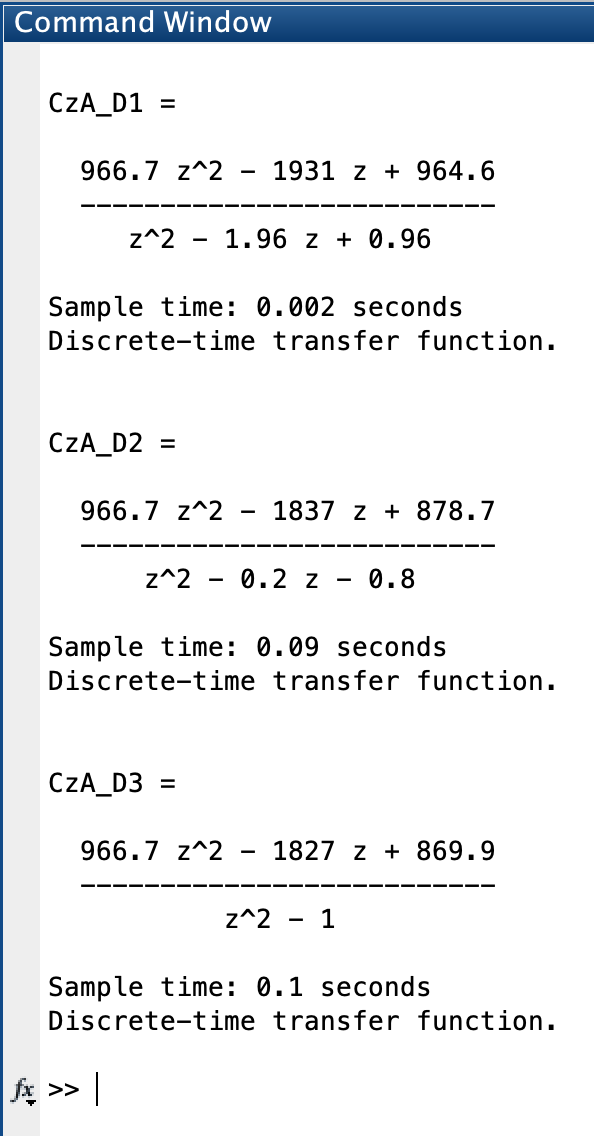
\includegraphics[width=4cm]{W3_CzA_DTFs.png}
    \caption{MATLAB outputs of simple approach emulated $C(z)$}
    \label{fig:CzA_DTFs}
\end{minipage}
\hspace{1cm}
\begin{minipage}{.6\textwidth}
    \centering
    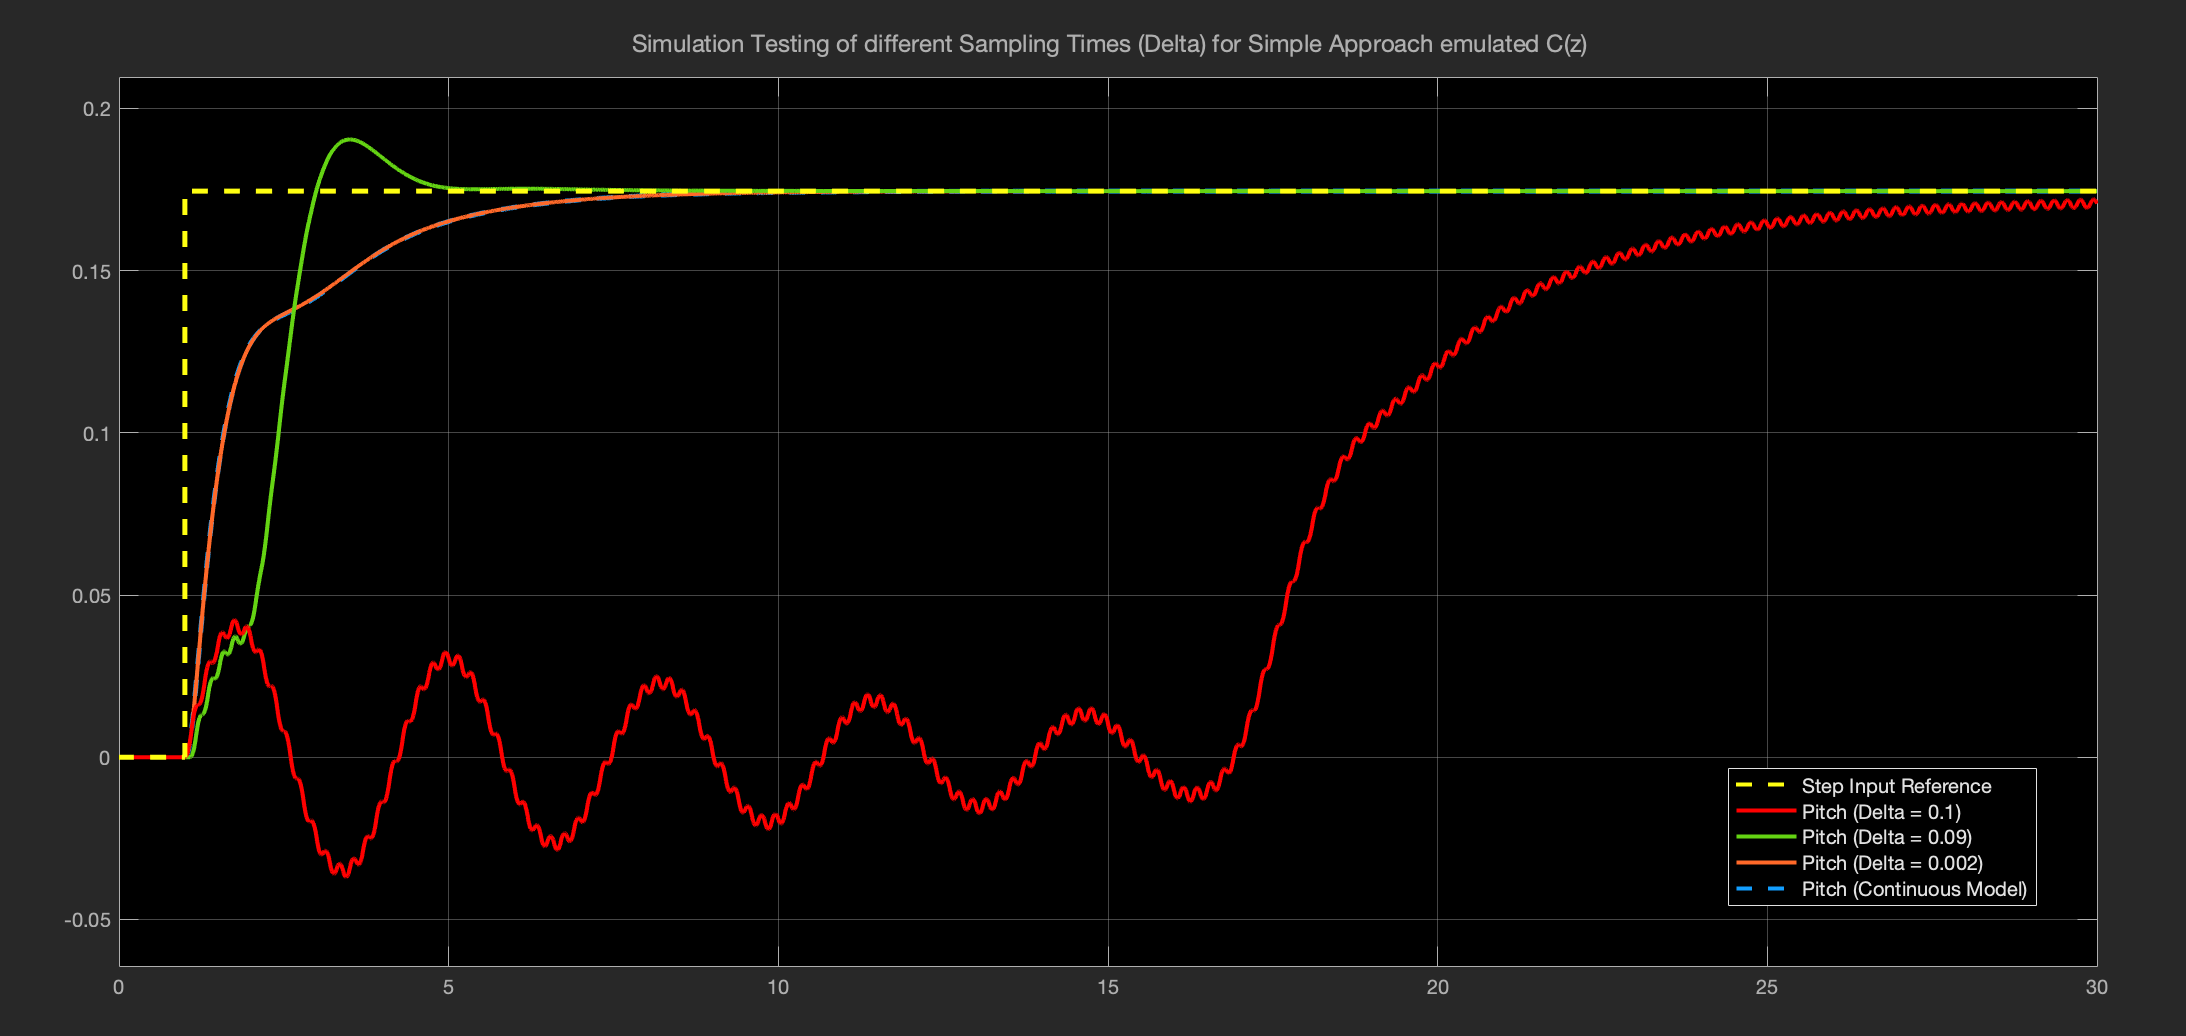
\includegraphics[width=10.5cm]{W3_CzA_DSim.png}
    \caption{Simulation results with simple controller emulation with $\Delta = 0.002, 0.09, 0.1$s}
    \label{fig:CzA_DSim}
\end{minipage}
\end{figure}

Likewise, the simple emulation discrete controllers were implemented in Quanser Aero with the sampling periods of $\Delta = 0.002, 0.09, 0.1$s. The respective system responses are shown in Figures \ref{fig:W3simple0}-\ref{fig:W3simple2}. 
\begin{figure}[H]
\begin{minipage}{.3\textwidth}
    \centering
    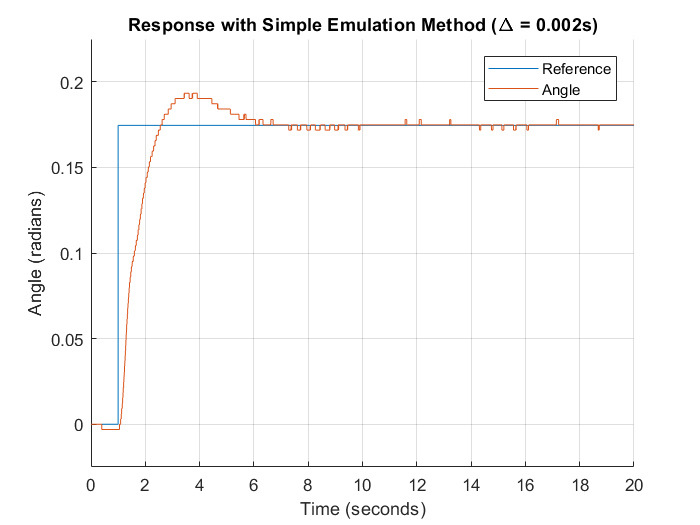
\includegraphics[width=5cm]{plots/Simple.png}
    \caption{Simple controller emulation with $\Delta = 0.002$s}
    \label{fig:W3simple0}
\end{minipage}
\hspace{0.5cm}
\begin{minipage}{.3\textwidth}
    \centering
    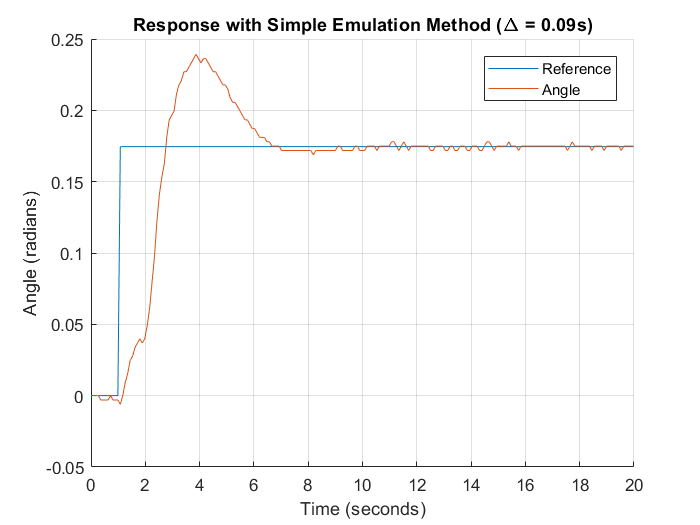
\includegraphics[width=5cm]{plots/Simple_0_09.png}
    \caption{\small{Simple controller emulation with $\Delta = 0.09$s}}
    \label{fig:W3simple1}
\end{minipage}
\hspace{0.5cm}
\begin{minipage}{.3\textwidth}
    \centering
    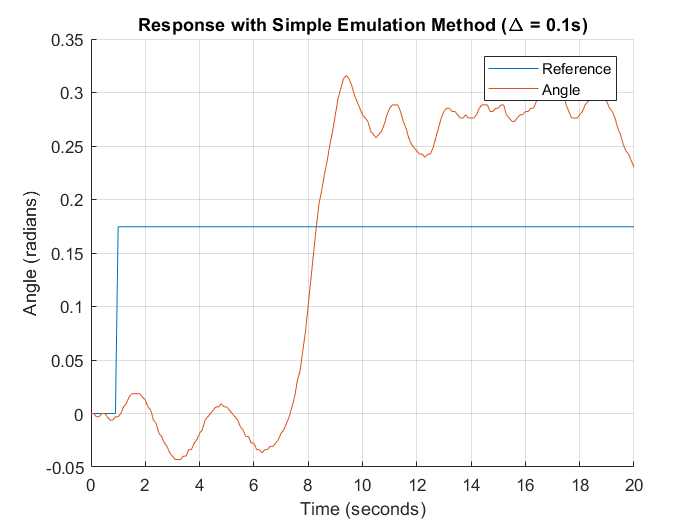
\includegraphics[width=5cm]{plots/Simple_0_1.png}
    \caption{\small{Simple controller emulation with $\Delta = 0.1$s}}
    \label{fig:W3simple2}
\end{minipage}
\end{figure}
In Figure \ref{fig:W3simple0} at $\Delta = 0.002$s, some overshoot is present in experimentation, though, the system stabilises at the reference pitch angle of $10^{\circ}$ after 8 seconds. This differs from our simulation response, which had no overshoot. The system remains stable at $\Delta = 0.09$s, albeit a large overshoot. It no longer tracks the reference and thus is unstable at $\Delta = 0.1$s echoing our simulation result. Again, there are discrepancies between the simulation and the experimental results, especially for $\Delta = 0.1$s, where the system does not overshoot in simulation. This is possibly due to intrinsic physical dynamics of the Quanser Aero not captured by our linearised model. 

\subsection{Step Invariant Discrete Controller}
The $C_B(z)$ for respective sampling periods of $\Delta = 0.002, 0.17, 0.18$s were obtained through MATLAB as seen in Figure \ref{fig:CzB_DTFs}. Like the simple approach discrete controllers, they were entered into our Simulink model as discrete time transfer functions with the corresponding sampling periods. The simulation results from Figure \ref{fig:CzB_DSim} show that with a step invariant emulated controller, the system becomes unstable at $\Delta = 0.17$s.

\begin{figure}[H]
\begin{minipage}{.3\textwidth}
    \centering
    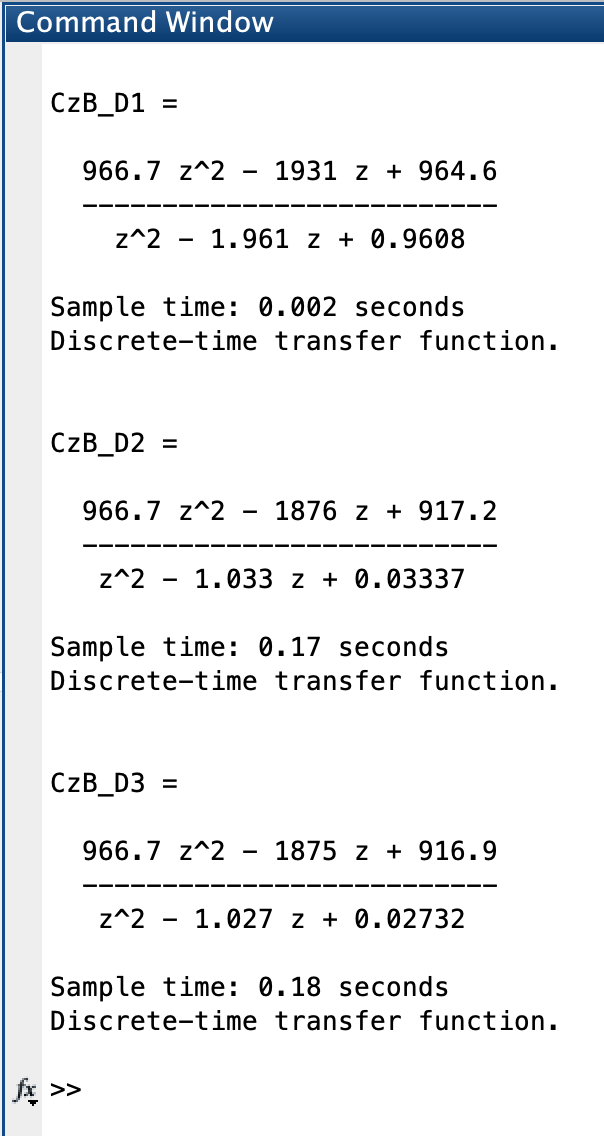
\includegraphics[width=4cm]{W3_CzB_DTFs.png}
    \caption{MATLAB outputs of step invariant emulated $C(z)$}
    \label{fig:CzB_DTFs}
\end{minipage}
\hspace{1cm}
\begin{minipage}{.6\textwidth}
    \centering
    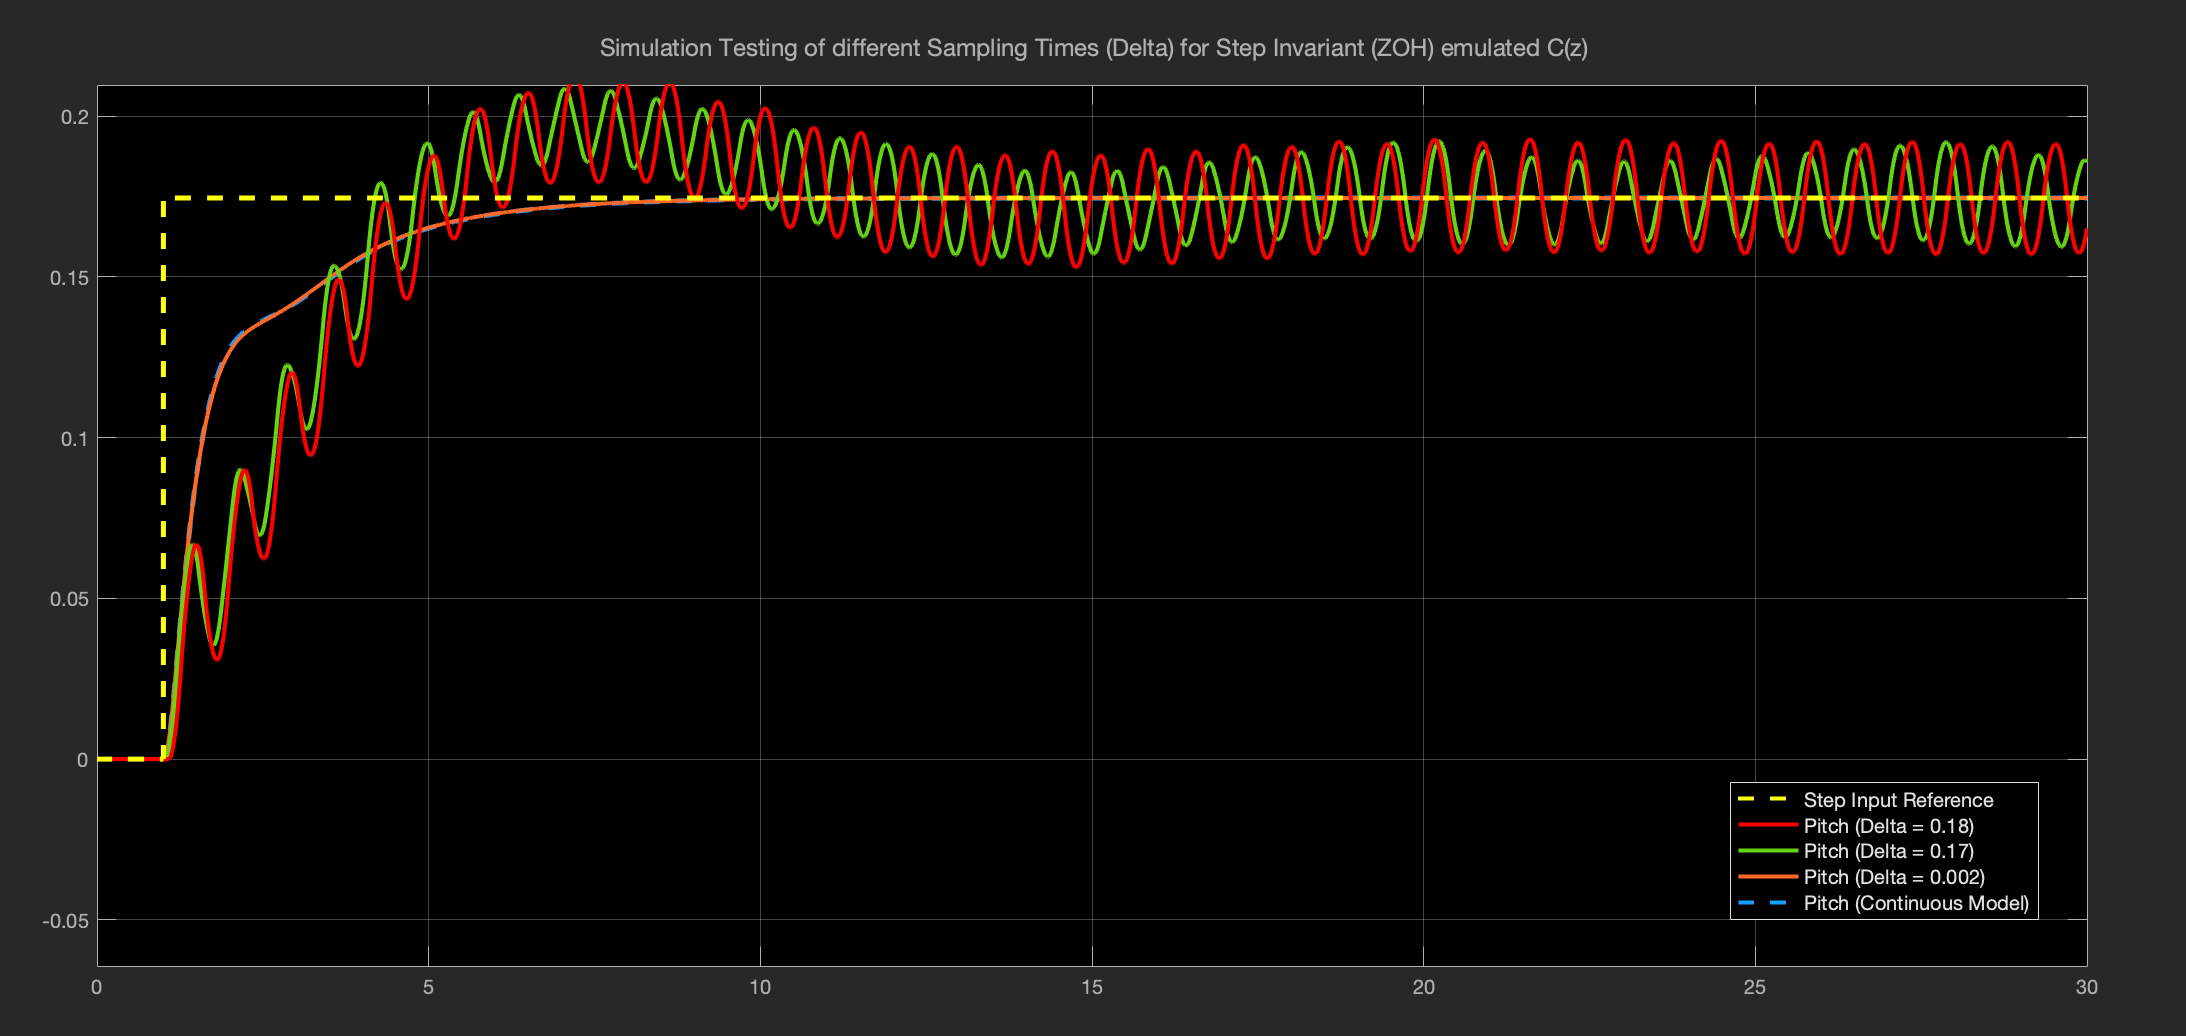
\includegraphics[width=10.5cm]{W3_CzB_DSim.png}
    \caption{Simulation results with step invariant emulation with $\Delta = 0.002, 0.17, 0.18$s}
    \label{fig:CzB_DSim}
\end{minipage}
\end{figure}

The Quanser Aero system responses are shown below in Figures \ref{fig:W3stepinvariant0}-\ref{fig:W3stepinvariant2} with respective sampling periods.

\begin{figure}[H]
\begin{minipage}{.3\textwidth}
    \centering
    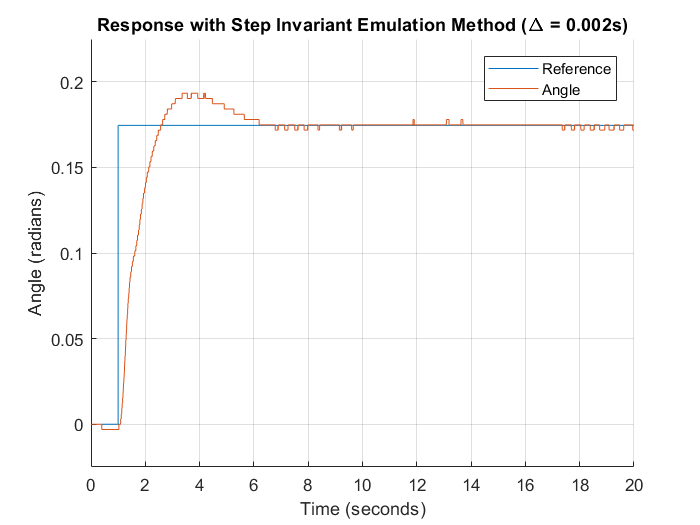
\includegraphics[width=5cm]{plots/StepInvariant.png}
    \caption{\small{ZOH controller emulation with $\Delta = 0.002$s}}
    \label{fig:W3stepinvariant0}
\end{minipage}
\hspace{0.5cm}
\begin{minipage}{.3\textwidth}
    \centering
    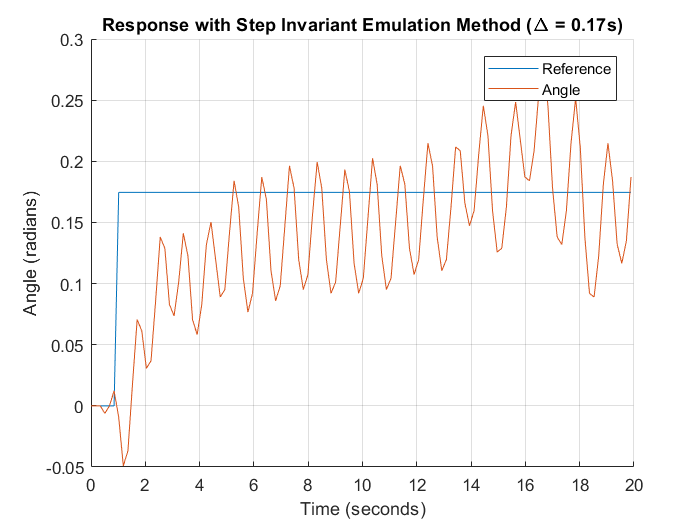
\includegraphics[width=5cm]{plots/StepInvariant_0_17.png}
    \caption{\small{ZOH controller emulation with $\Delta = 0.17$s}}
    \label{fig:W3stepinvariant1}
\end{minipage}
\hspace{0.5cm}
\begin{minipage}{.3\textwidth}
    \centering
    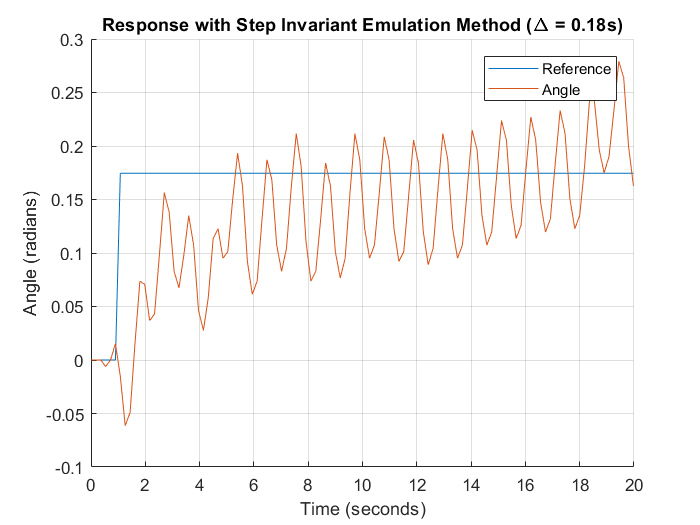
\includegraphics[width=5cm]{plots/StepInvariant_0_18.png}
    \caption{\small{ZOH controller emulation with $\Delta = 0.18$s}}
    \label{fig:W3stepinvariant2}
\end{minipage}
\end{figure}

The closed loop response with the step invariant (ZOH) emulation method at $\Delta = 0.002$s is almost equivalent to that with simple approach emulation Quanser Aero response: exhibiting the same overshoot properties and settling to the reference around $8$ seconds. The empirical response at $\Delta = 0.17$s sampling rate, shown in Figure \ref{fig:W3stepinvariant1}, sees heavy oscillations and the system struggling to track the reference around the 16 second mark. As such, this system can be described as unstable at this sampling rate which matches our simulation results. Upping this period slightly to $\Delta = 0.18$s, shown in Figure \ref{fig:W3stepinvariant2}, shows a similar response but with reference tracking lost at around 18 seconds. In both cases, there was no early overshoot as there was in our simulations. Again, differences with the simulation results could be due to intrinsic physical dynamics not captured by our simulation model.

\subsection{Bilinear with Pre-warping Discrete Controller}
All $C_C(z)$ for the sampling periods of $\Delta = 0.002, 0.257, 0.263$s were obtained through MATLAB as seen in Figure \ref{fig:CzC_DTFs}. Again, they were entered into our Simulink model as discrete time transfer functions with corresponding sampling periods. The simulation results from Figure \ref{fig:CzC_DSim} show that with a bilinear with pre-warping emulated controller, the system becomes fully unstable at $\Delta = 0.263$s.

\begin{figure}[H]
\begin{minipage}{.3\textwidth}
    \centering
    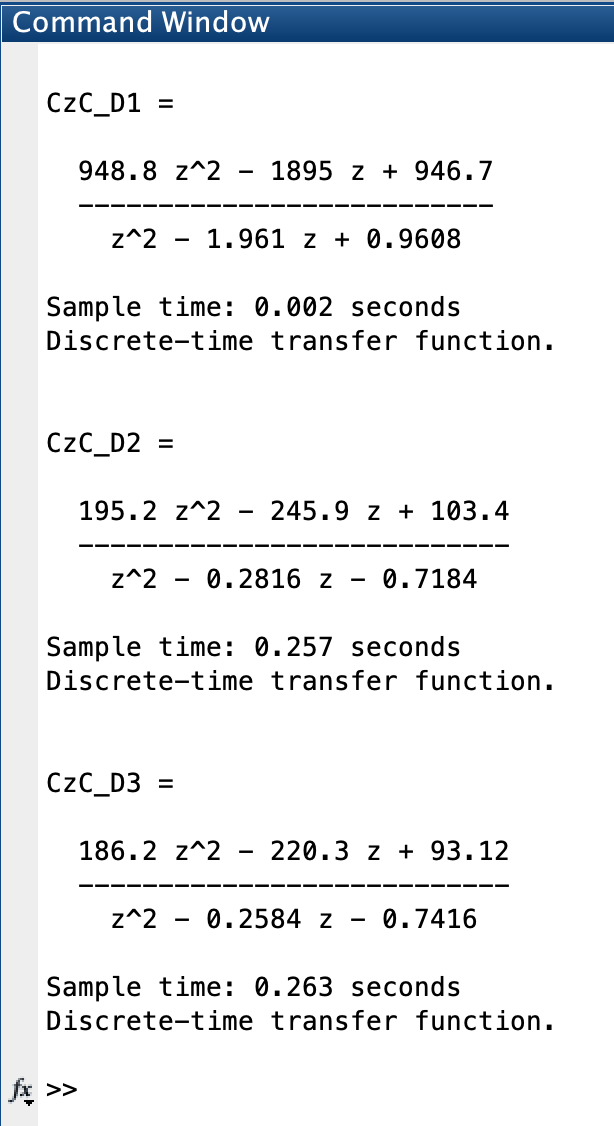
\includegraphics[width=4cm]{W3_CzC_DTFs.png}
    \caption{MATLAB outputs of bilinear emulated $C(z)$}
    \label{fig:CzC_DTFs}
\end{minipage}
\hspace{1cm}
\begin{minipage}{.6\textwidth}
    \centering
    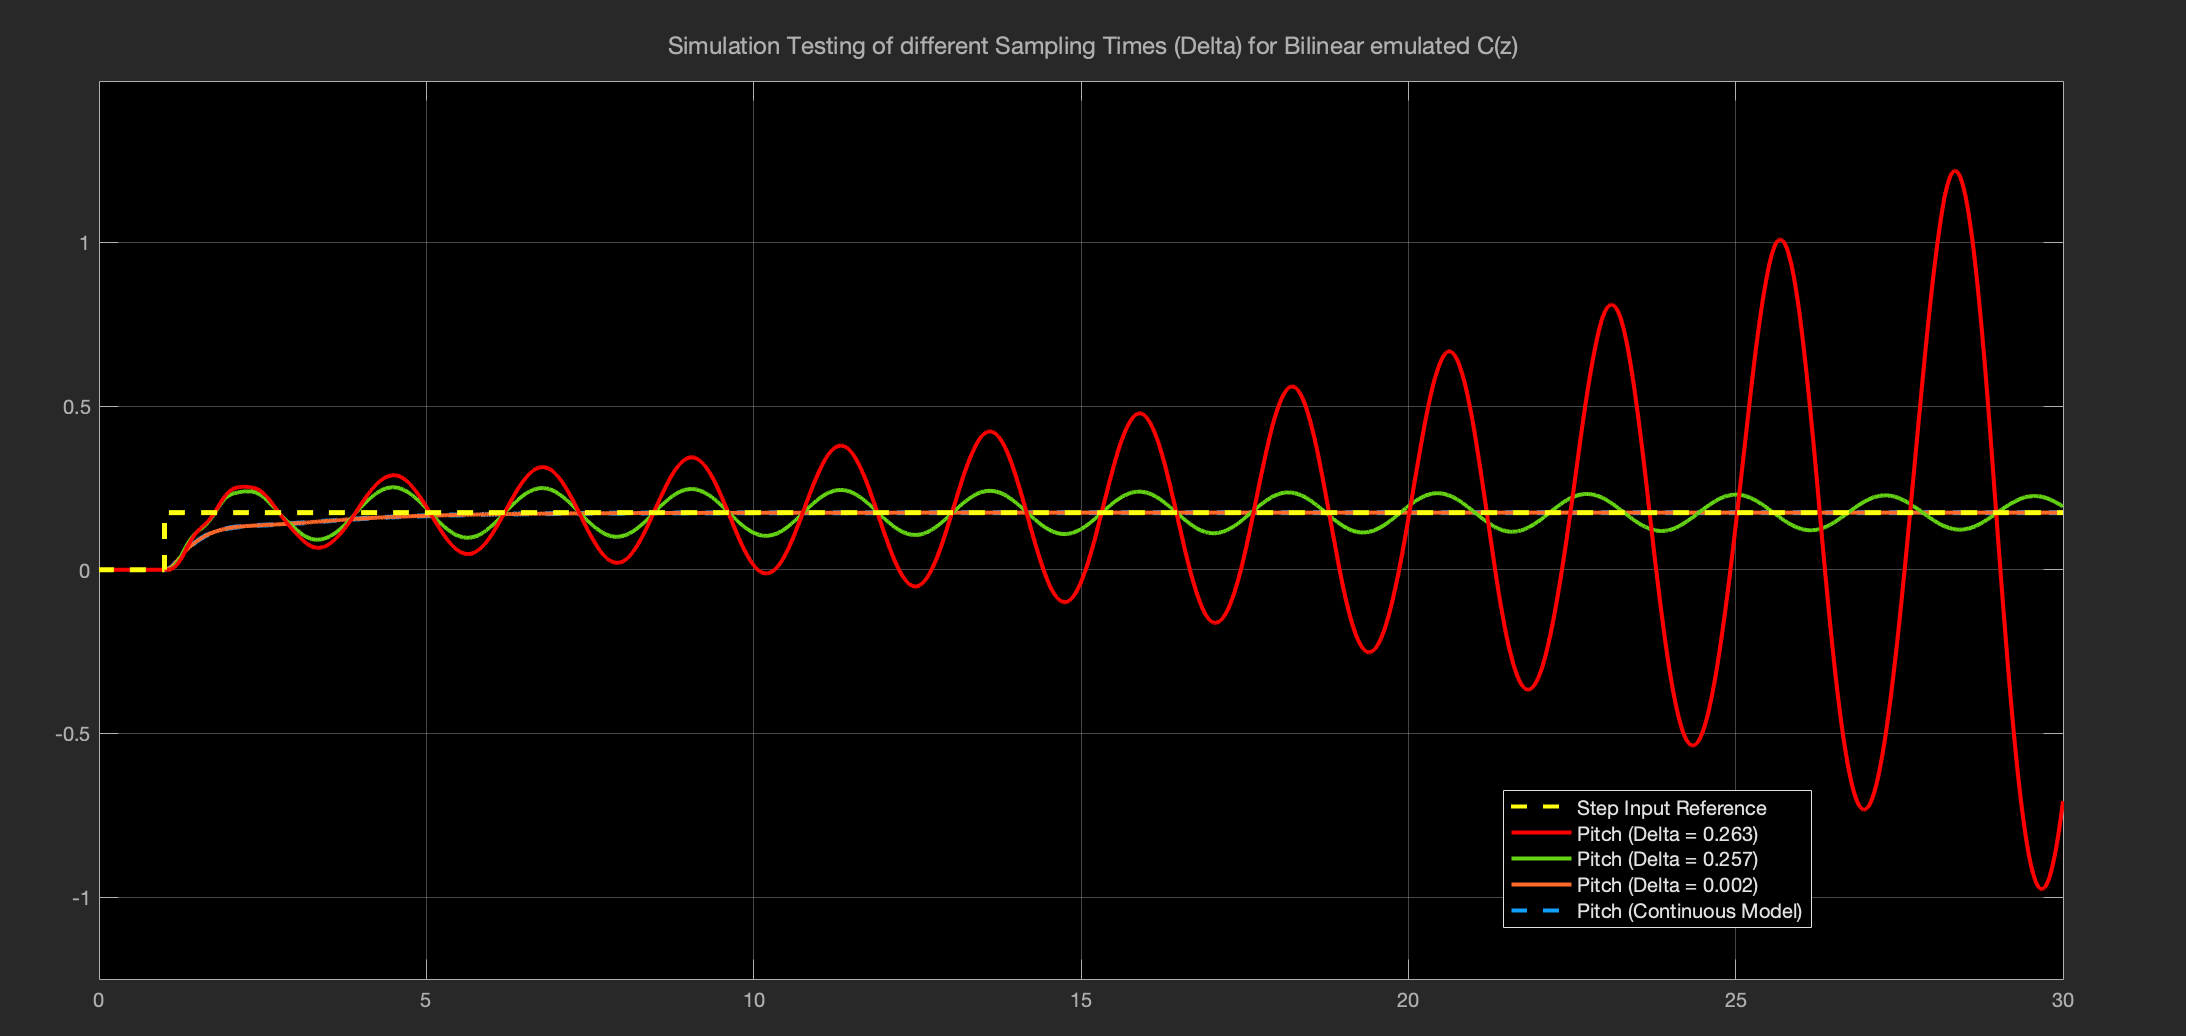
\includegraphics[width=10.5cm]{W3_CzC_DSim.png}
    \caption{Simulation results with bilinear emulation with $\Delta = 0.002, 0.257, 0.263$s}
    \label{fig:CzC_DSim}
\end{minipage}
\end{figure}

The Quanser Aero step responses for respective sampling periods for $C_C(z)$ are shown in Figures \ref{fig:W3bilinear0}-\ref{fig:W3bilinear2}.

\begin{figure}[H]
\begin{minipage}{.3\textwidth}
    \centering
    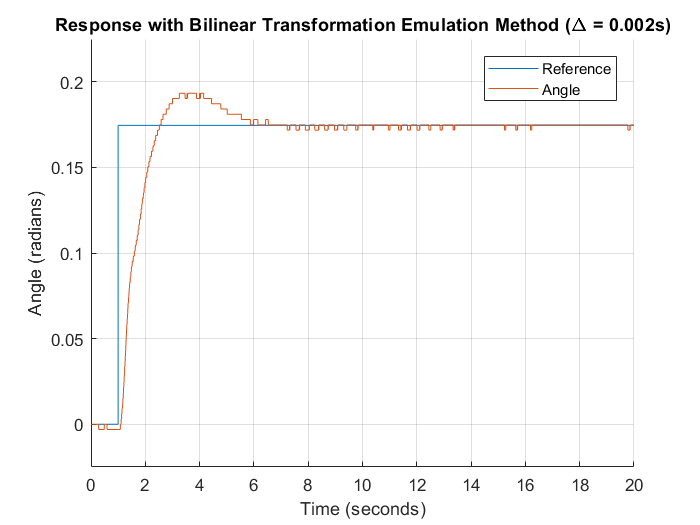
\includegraphics[width=5cm]{plots/Bilinear.png}
    \caption{\small{Bilinear controller emulation with $\Delta = 0.002$s}}
    \label{fig:W3bilinear0}
\end{minipage}
\hspace{0.5cm}
\begin{minipage}{.3\textwidth}
    \centering
    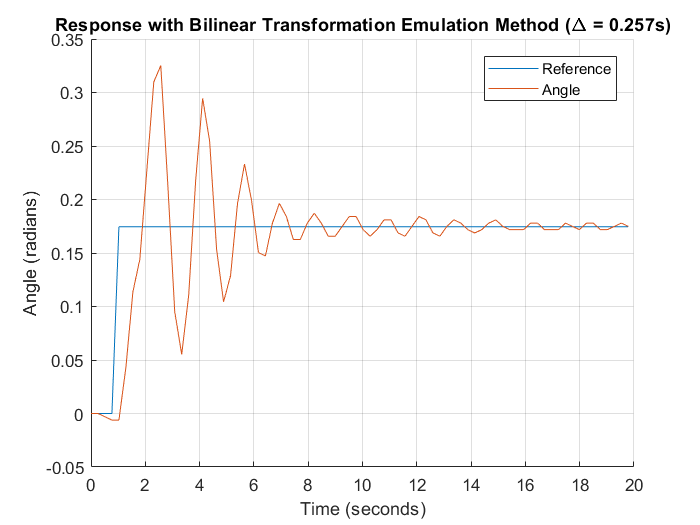
\includegraphics[width=5cm]{plots/Bilinear_0_257.png}
    \caption{\small{Bilinear controller emulation with $\Delta = 0.257$s}}
    \label{fig:W3bilinear1}
\end{minipage}
\hspace{0.5cm}
\begin{minipage}{.3\textwidth}
    \centering
    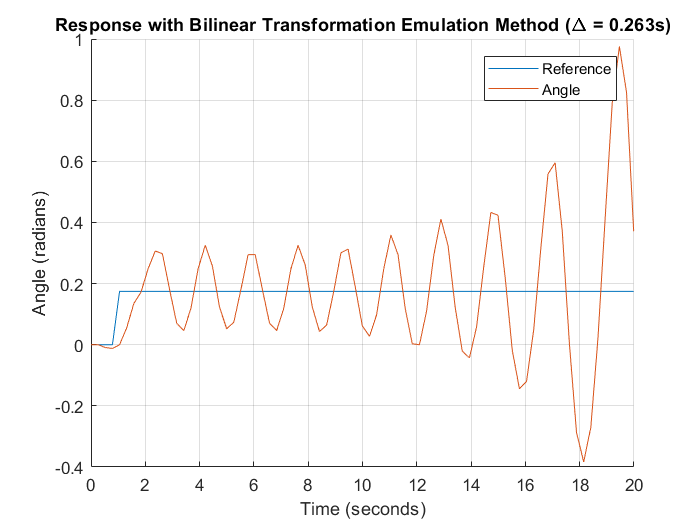
\includegraphics[width=5cm]{plots/Bilinear_0_263.png}
    \caption{\small{Bilinear controller emulation with $\Delta = 0.263$s}}
    \label{fig:W3bilinear2}
\end{minipage}
\end{figure}
For $\Delta = 0.002$s, the response is very similar to that of the simple approach and step invariant emulated controllers with a minor overshoot. This may be due to a sampling period too small to differentiate between the three methods. Simulations indicated that $\Delta = 0.257$s would approach an unstable system. In practice, at this sampling period the system exhibited heavy initial oscillations though remained stable and settled. This is shown in Figure \ref{fig:W3bilinear1}. Finally at $\Delta = 0.263$s, the system becomes unstable, as in Figure \ref{fig:W3bilinear2} and matches our simulation results, where the oscillations diverge. Bilinear emulation allowed the largest sampling period before system instability of the three emulation methods.

%%%%% DESIGN PI CONTROLLER %%%%%%
\section{Design and Simulation of a Discrete PI Controller}
From our experimental testing we decided that the bilinear transform gave a more robust system allowing for a larger sampling period to trigger system instability. We decided to design our discrete PI controller for the $G(z)$ also obtained through bilinear emulation at the sampling period of $\Delta = 0.263$s. Substituting $\Delta$ into our expression found in Eq.\ref{eq:GCz} under Section \ref{section:calcs}, we get the following in MATLAB in Figure \ref{fig:GzC_DTF}. The discretised system's root locus plot is shown in Figure \ref{fig:GzC_rlocus}.

\begin{figure}[H]
    \begin{minipage}{.5\textwidth}
    \centering
    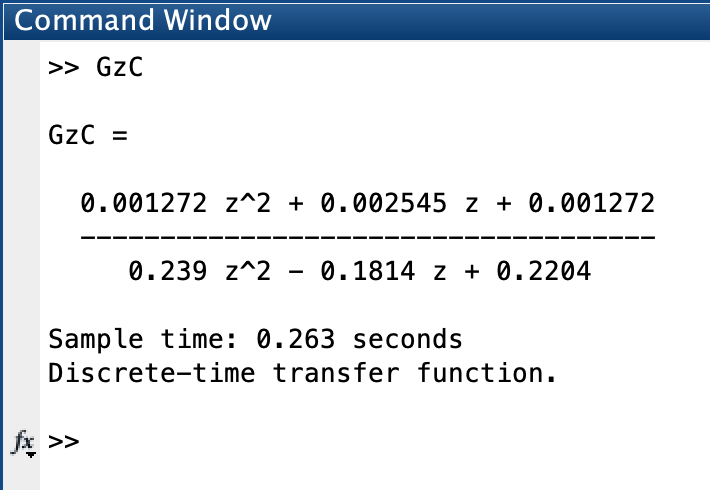
\includegraphics[width=7cm]{W3_GzC_DTF.png}
    \caption{MATLAB output of $G_C(z)$ at $\Delta = 0.263$s}
    \label{fig:GzC_DTF}
    \end{minipage}%
    \begin{minipage}{.5\textwidth}
    \centering
    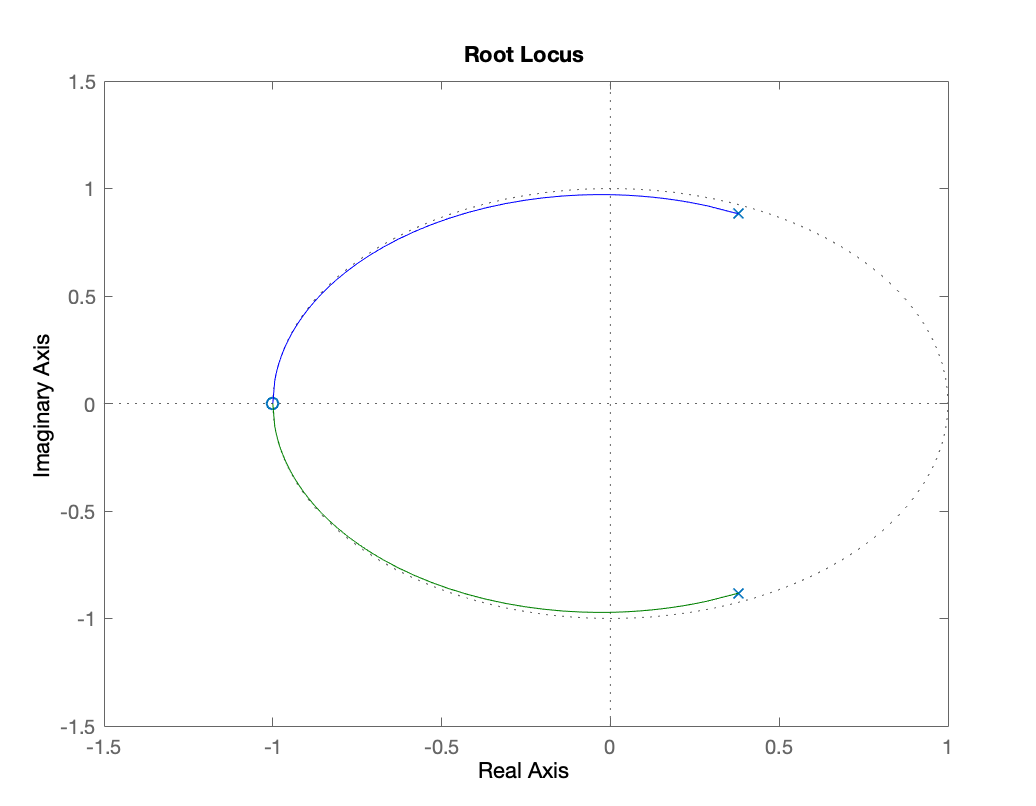
\includegraphics[width=8cm]{W3_GzC_rlocus.png}
    \caption{Root locus plot of $G_C(z)$}
    \label{fig:GzC_rlocus}
     \end{minipage}%
\end{figure}

To design a PI controller $C(z) = k_d + \frac{k_i}{z}$, we attempted to set $k_i=0.1$ and tune $k_p$, however the results from this showed nothing but heavy oscillations even at high gains of $k_d = 200$. We instead initially set the PI gains to arbitrary values in order to gain an understanding of the response of the simulated system and tuned it from there. With the gains set to $k_p = 1$ and $k_i = 10$, the simulated step response of the system is shown in Figure \ref{fig:W3discreteplant0}. We noted that by increasing the proportional gain to $k_p = 4$, the settling time did not seem to reduce and the only affect it had was an increase in response oscillations. \\

\begin{figure}[H]
\begin{minipage}{.5\textwidth}
    \centering
    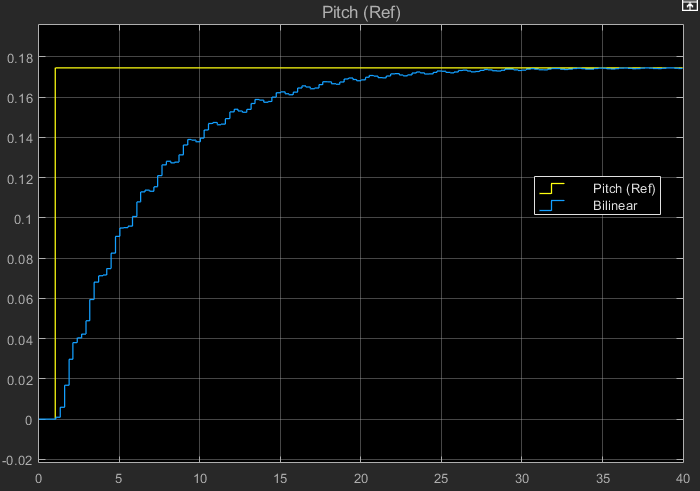
\includegraphics[width=8cm]{plots/discreteplant_sim_ki10_kp1.png}
    \caption{\small{Response with $k_{p}=1, k_{i}=10$}}
    \label{fig:W3discreteplant0}
\end{minipage}%
\begin{minipage}{.5\textwidth}
    \centering
    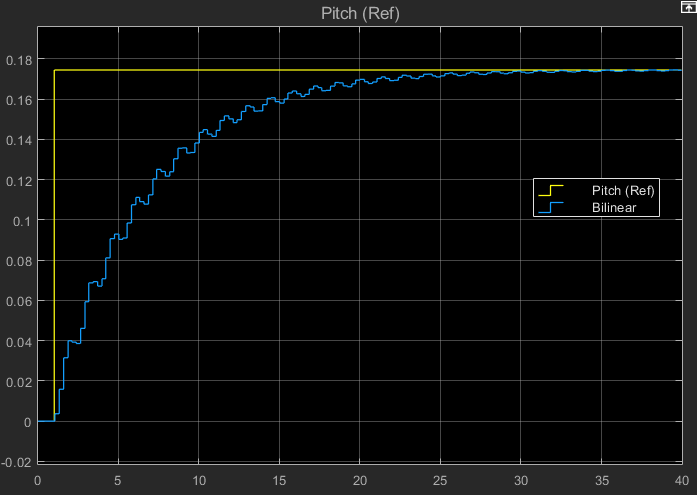
\includegraphics[width=8cm]{plots/discreteplant_sim_ki10_kp4.png}
    \caption{\small{Response with $k_{p}=4, k_{i}=10$}}
    \label{fig:W3discreteplant1}
\end{minipage}
\end{figure}

From here we attempted some tuning methods including Ziegler–Nichols as well as Simulink in-built PID autotuning algorithms. The resulting gains derived from one of these methods was $k_p = 0.6676$ and $k_i = 5.1955$ and the response is shown in Figure \ref{fig:W3discreteplant2}. As evident, the response seemed slower than with the arbitrary values as assigned in Figure \ref{fig:W3discreteplant0}, and thus these were the values initially implemented in Quanser Aero experimentally. After the implementation as described in the following section, we returned to simulations with the final designed PI controller: $k_p = 8$ and $k_i = 5.7595$. In simulations, the response is stable though exhibits oscillation, and this may be due to an error in simulations or a difference in the physical system not captured by the model. \\

\begin{figure}[H]
\begin{minipage}{.5\textwidth}
    \centering
    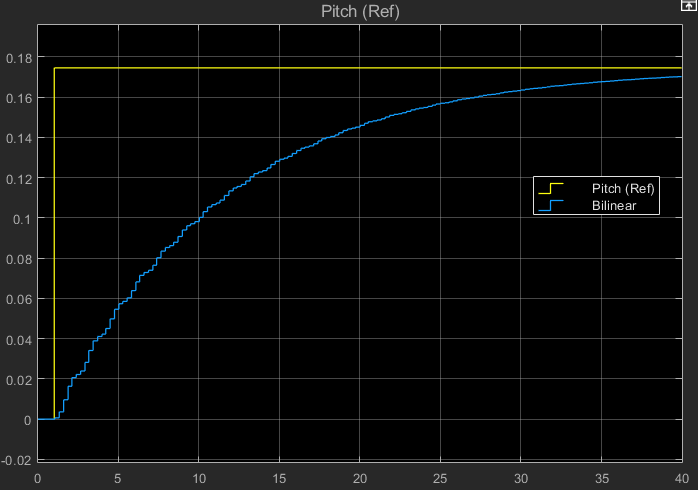
\includegraphics[width=8cm]{plots/discreteplant_sim_ki5_1955_kp0_6676.png}
    \caption{\small{Response with $k_{p}=0.6676, k_{i}=5.1955$}}
    \label{fig:W3discreteplant2}
\end{minipage}%
\begin{minipage}{.5\textwidth}
    \centering
    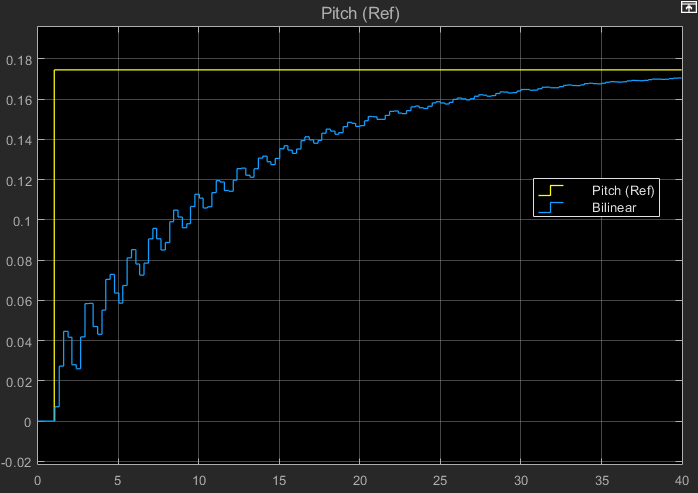
\includegraphics[width=8cm]{plots/discreteplant_sim_ki5_7595_kp8.png}
    \caption{\small{Response with $k_{p}=8, k_{i}=5.7595$}}
    \label{fig:W3discreteplant3}
\end{minipage}
\end{figure}

%%%%%%%%%%%% BEGIN IMPLEMENTATION SECTION %%%%%%%%%%%%%%%%
\section{Implementation of Discrete PI Controllers on G(z)}
One of the proposed PI controllers derived in simulations was with $k_{p} = 1$ and $k_i = 10$. This PI controller was implemented in Quanser Aero and the results are shown in Figure \ref{fig:W3discrete0}. As evident, the system is highly unstable and does not converge. Another of the simulation derived PI controllers with $k_{p} = 0.6676$ and $k_i = 5.1955$ was then implemented and the response is as in Figure \ref{fig:W3discrete1}. Here the response seems closely stable in that it tracks the reference but heavy oscillations are present throughout. We therefore continued tuning the controller based on real-time responses from the Quanser Aero.\\

\begin{figure}[H]
\begin{minipage}{.5\textwidth}
    \centering
    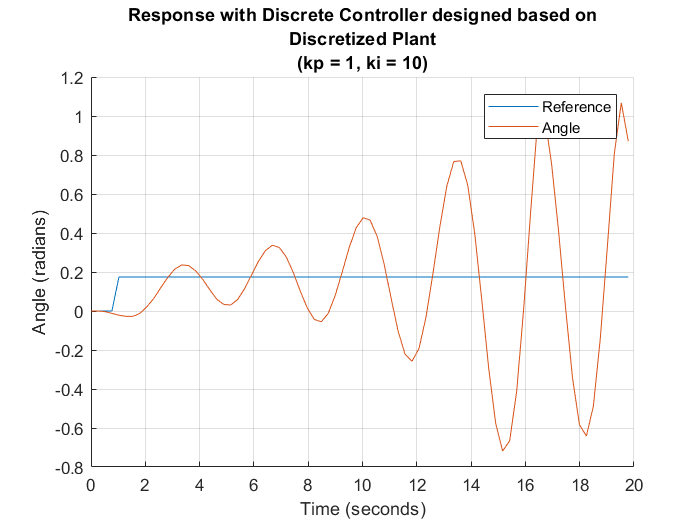
\includegraphics[width=8cm]{plots/Discrete_1_10.png}
    \caption{\small{Response with designed discrete controller}}
    \label{fig:W3discrete0}
\end{minipage}%
\begin{minipage}{.5\textwidth}
    \centering
    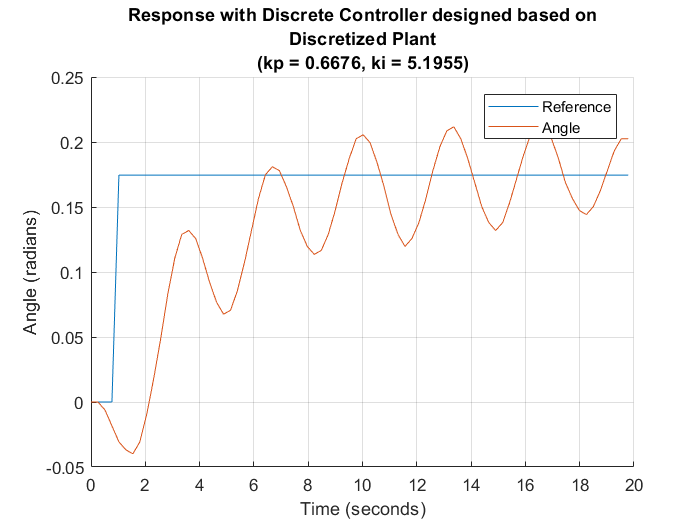
\includegraphics[width=8cm]{plots/Discrete_0_6676_5_1955.png}
    \caption{\small{Response with designed discrete controller}}
    \label{fig:W3discrete1}
\end{minipage}
\end{figure}

Finally, after controller tuning based on Ziegler–Nichols (altering $K_u$, the ultimate gain and $T_u$, the oscillation period - both derived through experimentation), the result is a response with minimal overshoots in the oscillations and convincing tracking as the oscillations subdues after 30s. This is shown in Figure \ref{fig:W3discrete2}. The Nyquist plot in Figure \ref{fig:Nyquist} of the closed loop sensitivity $L = GC$, gives one anticlockwise loop showing that the system is stable.

\begin{figure}[H]
    \begin{minipage}{.5\textwidth}
    \centering
    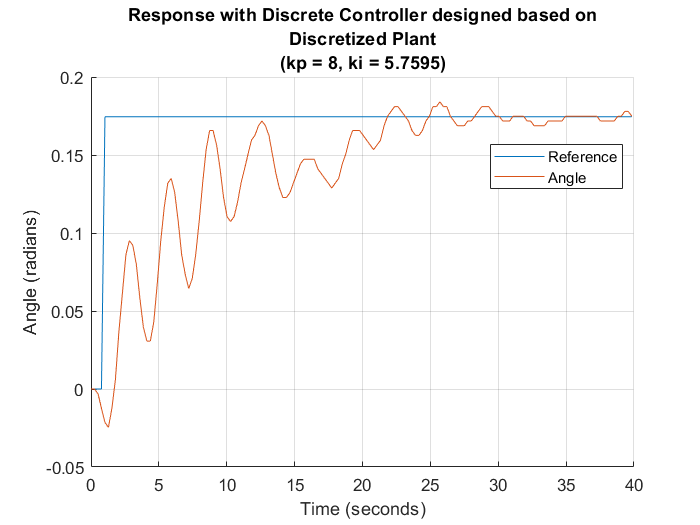
\includegraphics[width=8cm]{plots/Discrete_8_5_7595.png}
    \caption{Response with designed discrete controller}
    \label{fig:W3discrete2}
    \end{minipage}%
    \hspace{0.5cm}
    \begin{minipage}{.5\textwidth}
    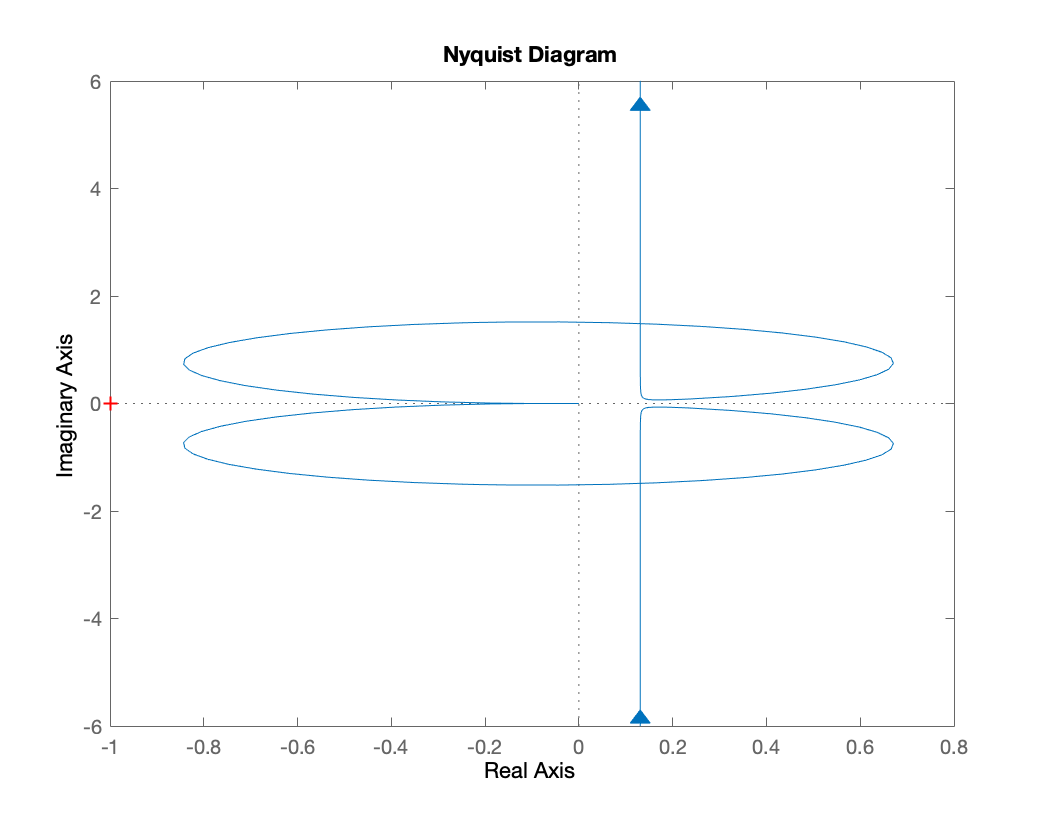
\includegraphics[width=8cm]{W3_Nyquist.png}
    \caption{Nyquist plot of $L = GC$}
    \label{fig:Nyquist}
    \end{minipage}
\end{figure}

Our final PI gains were $k_{p} = 8$ and $k_i = 5.7595$. Giving the discrete PI controller as,
\begin{equation}\label{eq:DPI}
    C_{PI}(z) = k_p + k_i \frac{\Delta}{z - 1} = 8 + \frac{1.5147}{z -1}
\end{equation}

%%%%%%%%%%%% BEGIN CONCLUSION %%%%%%%%%%%%%%%%
\section{Conclusions}
Through simulating and testing the various emulation methods to discretise our designed continuous controller $C(s)$ to $C(z)$, it seemed that in this scenario, with a small enough sampling period, the three methods all showed step responses close to that of the continuous controller system. With increased sampling periods, the emulated controllers showed instability in the order of 1. simple approach, 2. step invariant, and 3. bilinear with pre-warping. This shows us that the bilinear emulated controller is more robust and has more leeway in the case of sampling restrictions. Our final responses including at unstable sampling periods can be seen in Figures \ref{fig:W3finalsimple} - \ref{fig:W3finalbilinear}. \\

\begin{figure}[H]
\begin{minipage}{.3\textwidth}
    \centering
    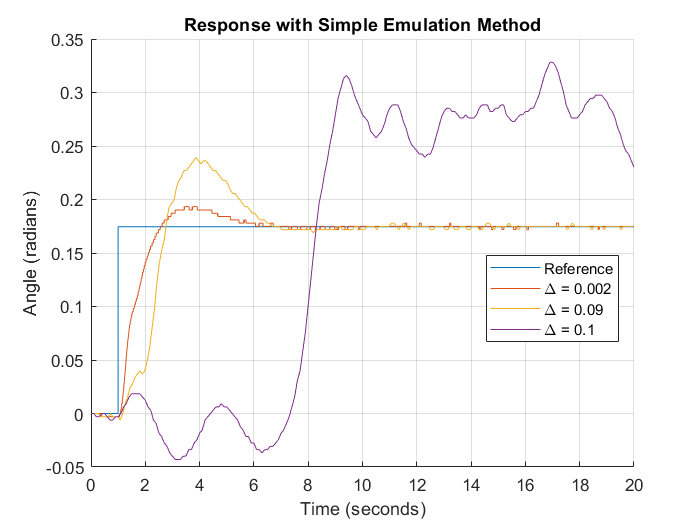
\includegraphics[width=5cm]{final_simple_emulation.png}
    \caption{\small{Simple controller emulation}}
    \label{fig:W3finalsimple}
\end{minipage}
\hspace{0.5cm}
\begin{minipage}{.3\textwidth}
    \centering
    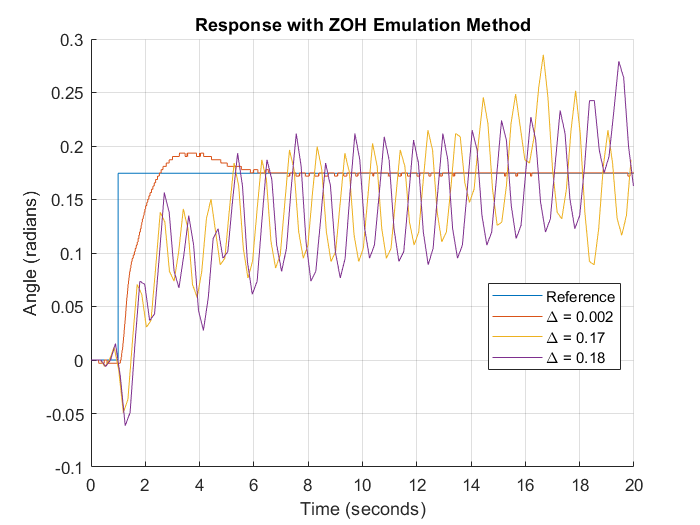
\includegraphics[width=5cm]{final_zoh_emulation.png}
    \caption{\small{Step invariant controller emulation}}
    \label{fig:W3finalzoh}
\end{minipage}
\hspace{0.5cm}
\begin{minipage}{.3\textwidth}
    \centering
    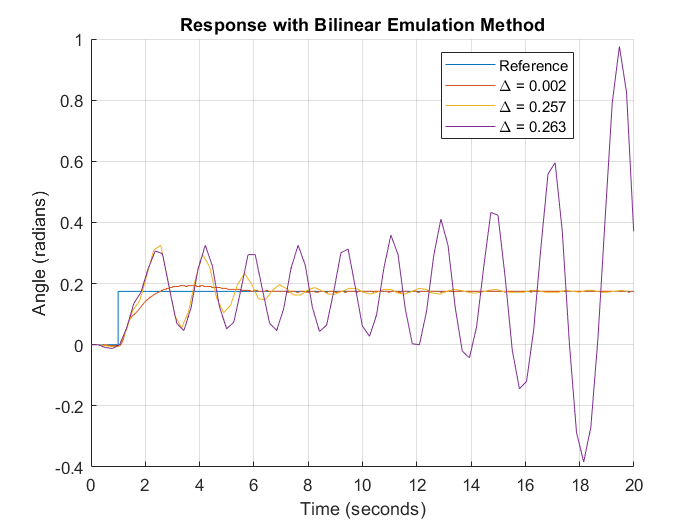
\includegraphics[width=5cm]{final_bilinear_emulation.png}
    \caption{\small{Bilinear controller emulation}}
    \label{fig:W3finalbilinear}
\end{minipage}
\end{figure}

Designing a discrete PI controller to stabilise an unstable discretised system $G(z)$ wasn't a straight forward job as oscillatory behaviour did not change significantly with $k_p$. Settling time was the compromise in our design results and the final tuned PI controlled system. Our PI controller to stabilise the plant was designed via a variety of controller tuning methods including Ziegler–Nichols, and the final physical Quanser Aero response of our final PI controller can be seen in Figure \ref{fig:W3discrete2}. Simulations of this same controller are as Figure \ref{fig:W3discreteplant3}, and it is noted that there are quite large discrepancies between the empirical response and the simulation response. This is again likely due to physical dynamics in the Quanser Aero system that are not captured by our models.

%% FINAL MARKING SCHEME CHECKOFFS %%

% (Section 2) Present details of all calculations for each of the \textbf{three emulation methods for different sampling periods}. 

% (Fig 2,7,12) 
%Provide on a single plot a comparison of simulations of step responses (different plot for each emulation method) with various sampling periods;

% (Fig 26,27,28)
%then provide the same plots for experiments with the same controller and the same sampling periods. 
% (Section 3)
%Present simulation and experimental results for the sampling periods at which the closed-loop becomes unstable.}\\

% (Fig 16)
%Provide the details of \textbf{plant discretization} for the chosen sampling period.
% (Section 4,5)
%Present the details of a discrete-time PI controller design. Provide simulation for a step response with the designed controller and comparison with a step response for Aero controlled with the same controller.}\\

%\colorbox{yellow}{Page limit: 10 pages. We have 1 more page to go. Appendix is full. 5/5}




\newpage
\section{Appendix}
\subsection{Simulink Models}
\begin{figure}[H]
    \centering
    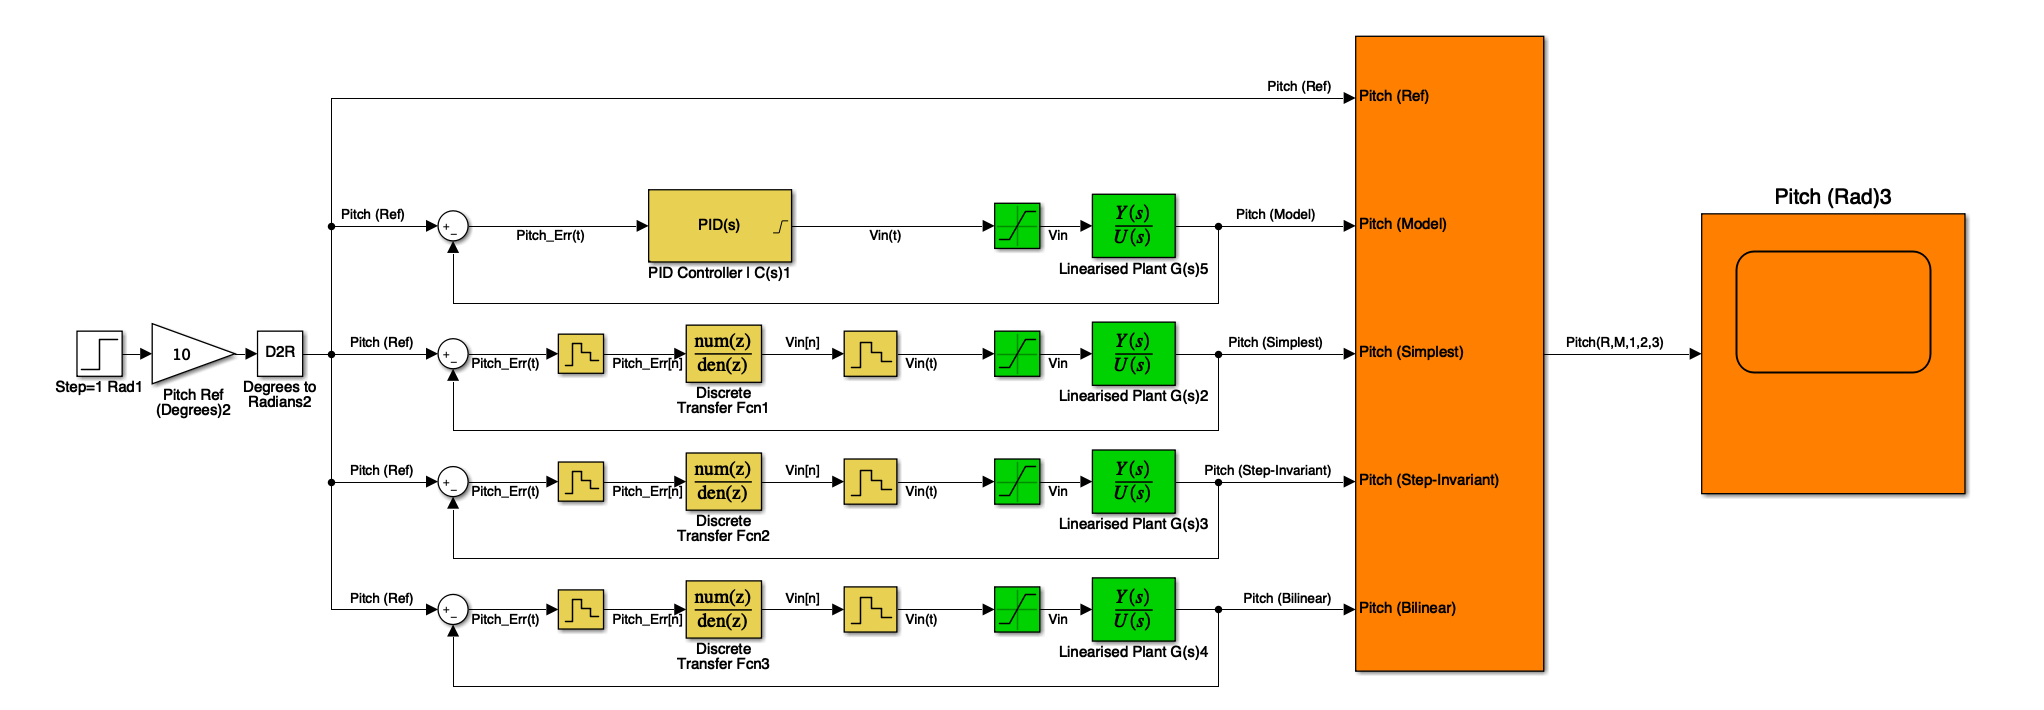
\includegraphics[scale=0.5]{W3_Simulink_Cz.png}
    \caption{Simulink model for testing Sampling Periods in Emulation}
    \label{fig:sims_Cz}
\end{figure}
\subsection{MATLAB Code}
\begin{lstlisting}[frame=single]
%% WS2 (Wk2-3)[2]:
%% Parameters:
% DEFAULT -- [ theta_ss (0.4) || ts (2.8) || tau_b (5.0) ].
%  - Fixed.
g = 9.81;       Mb = 1.15;      Dt = 0.158;     Dm = 0.0071;    V_in = 24;
%  - Calculate... Thrust Const / Moment of Inertia / Viscous Damping Coeff.
theta_ss = 0.455;                   Kth = Mb*g*Dm*sin(theta_ss)/(V_in*Dt);
ts = 3.215;     w_n = 2*pi/ts;      Jp_sys = Mb*Dm*g/(w_n^2);
tau_b = 5.80;                       Dp = Jp_sys/tau_b;

%% State Space:
A = [ 0 1 ; -(Mb*g*Dm)/Jp_sys -Dp/Jp_sys ]   % A = [0,1;-3.8194,-0.17241];
B = [ 0 ; Kth*Dt/Jp_sys ]                    % B = [0;0.0699371899388020];
C = [ 1 0 ]
D = [ 0 ]                        

%% Plant Transfer Function:
% G_num = [ 0 0 0.0699 ] // G_den = [ 1.0000 0.1724 3.8194 ]
% Gs = b0 / ( s^2 + a1 s + a0 );
[G_num, G_den] = ss2tf(A,B,C,D);    Gs = tf( G_num, G_den )
b0 = G_num(3);    a1 = G_den(2);    a0 = G_den(3);

%% WS2 (Wk2-3)[3]:

%% 2.1 SECOND ORDER SYSTEM APPROXIMATION.
tmax = 2.459;    tp = tmax-1;
ymax = 0.533;    yf = 0.269;
PO = 100*(ymax-yf)/yf;
DampRatio = 1 / sqrt( 1 + ( pi/log(100/PO) )^2 );
w_n = pi / (tp * sqrt(1 - DampRatio^2) );

A0 = yf*w_n^2;
B2 = 1;     B1 = 2*DampRatio*w_n;       B0 = w_n^2*(1-yf);
kp = 1;     ki = 0;     kd = 0;

%% 2.2 Calculate PID Gains.
%  Controller calculations here.

p0 = 1;         DampRatio = 1;  % Critically Damped.
kp = (w_n^2 + 2*DampRatio*w_n*p0 - a0) / b0
ki = (w_n^2*p0) / b0
kd = (2*DampRatio*w_n + p0 - a1) / b0

%% Ziegler-Nichols Tuning "No Overshoot".
%  https://en.wikipedia.org/wiki/Ziegler%E2%80%93Nichols_method

% Ultimate Gain | Oscillation Period.
Ku = 20;    Tu = 2.453;

% INITIAL. [No Overshoot Method]
%kp = Ku/5;  ki = (2/5)*Ku/Tu;   kd = Ku*Tu/15;

% FINAL. Adjusted Kp and Ki.
%kp = Ku/5.5;    ki = (2.2/5)*Ku/Tu  kd = Ku*Tu/15

% REMOVE GAIN=7 BLOCK.
kp = 14 * Ku/5.5
ki = 14 * (2.2/5)*Ku/Tu
kd = 14 * Ku*Tu/15

%% WS3 (Wk4-5)[4]:

%% %% Define everything I'll need:
%% Controller:
%  - Cs = kp + ki/s + kd N s / ( s + N )
s = tf('s');        N = 20;
Cs = kp + ki/s + kd*N*s/(s+N);

%% Discrete variable:
%  - Default Sampling Period (2ms).
Delta = 0.1;
z = tf('z', Delta);
gamma = (z-1)/Delta;

%% %% RESULTS:
%% EMULATION [Plug and Play]:
% - CzA YES     UNSTABLE @ Delta = 0.100s
% - CzB YES     UNSTABLE @ Delta = 0.170s
% - CzC YES     UNSTABLE @ Delta = 0.257s

%% (1) Simplest:
%  - CzA = { Cs |s=gamma } |gamma=(z-1)/Delta
%CzA = kp + ki/gamma + kd*N*gamma/(gamma + N)
CzA = kp + ki*Delta/(z-1) + kd*N*(z-1)/(z-1+N*Delta)
[Num_CzA, Den_CzA] = tfdata(CzA, 'v');

%% (2) Step-Invariant:
%  - CzB = (1-z^-1)* Ztf{ L^-1{Cs/s}|t=n*Delta }
CzB = kp + ki*Delta/(z-1) + kd*N*(z-1)/(z-exp(-N*Delta))
[Num_CzB, Den_CzB] = tfdata(CzB, 'v');

%% (3) Bilinear Transform:
%  - CzC = { Cs |s=alpha*gamma/(0.5*Delta*Gamma+1) } |gamma=(z-1)/Delta
%  - Hence, s = 2*alpha*(z-1)/(Delta*(z+1))

figure; bode( 1 / (1 + Gs*Cs) );  grid on;
w_a = 9.684;    % (w*, Mag) = (9.684 rad, 1.152).
alpha = (w_a*Delta/2) * sin(w_a*Delta)/(1-cos(w_a*Delta))
alpha = (w_a*Delta/2) * cot(w_a*Delta/2)

CzC = kp + ki*Delta/(2*alpha)*(z+1)/(z-1) + kd*N*2*alpha/(N*Delta+2*alpha)*(z-1) / (z + (Delta*N-2*alpha)/(Delta*N+2*alpha) )
[Num_CzC, Den_CzC] = tfdata(CzC, 'v');


%% WS3 (Wk4-5)[5]:
%% Gs = b0 / ( s^2 + a1 s + a0 );
%  [G_num, G_den] = ss2tf(A,B,C,D);    Gs = tf( G_num, G_den )
%  b0 = G_num(3);    a1 = G_den(2);    a0 = G_den(3);

%% EMULATION [Plug and Play]:
% Cz = Kp + Ki*Ts/(z-1);
% - GzA     UNSTABLE @ Delta = 0.100s
% - GzB     UNSTABLE @ Delta = 0.170s
% - GzC     UNSTABLE @ Delta = 0.257s

%% (1) Simplest:
%  - GzA = { Gs |s=gamma } |gamma=(z-1)/Delta
DeltaA = 0.100;     z = tf('z', DeltaA);
GzA = b0*DeltaA^2 / ( z^2 + (a1*DeltaA-2)*z + (1-a1*DeltaA+a0*DeltaA^2) )
[Num_GzA, Den_GzA] = tfdata(GzA, 'v');
KiA = 0.1;     KpA = 1;

%% (2) Step-Invariant:
%  - GzB = (1-z^-1)* Ztf{ L^-1{Gs/s}|t=n*Delta }
DeltaB = 0.170;     z = tf('z', DeltaB);
[Gss_num, Gss_den] = tfdata(Gs/s, 'v')
[R,P,K] = residue(Gss_num, Gss_den)
%[Num_GzB, Den_GzB] = tfdata(GzB, 'v');

%% (3) Bilinear Transform:
%  - GzC = { Gs |s=alpha*gamma/(0.5*Delta*Gamma+1) } |gamma=(z-1)/Delta
%  - Hence, s = GzC = { Gs } | s=2*alpha*(z-1)/(Delta*(z+1))
DeltaC = 0.263;     z = tf('z', DeltaC);
figure; bode( 1 / (1 + Gs*Cs) );  grid on;
w_a = 9.684;    % (w*, Mag) = (9.684 rad, 1.152).
alphaC = (w_a*DeltaC/2) * sin(w_a*DeltaC)/(1-cos(w_a*DeltaC))
alphaC = (w_a*DeltaC/2) * cot(w_a*DeltaC/2)

s_bi = ( 2*alphaC*(z-1) ) / ( DeltaC*(z+1) );
GzC = b0 / ( s_bi^2 + a1*s_bi + a0 )
[pole,zero] = pzmap(GzC)

%GzC = b0*DeltaC^2*(z+1)^2 / ( 4*alphaC^2*(z-1)^2 + a1*2*alphaC*DeltaC*(z^2-1) + a0*DeltaC*(z+1)^2 )
GzC = b0*(z+1)^2 / ( (2*alphaC*(z-1)/DeltaC)^2 + a1*(2*alphaC*(z^2-1)/DeltaC) + a0*(z+1)^2 )
[Num_GzC, Den_GzC] = tfdata(GzC, 'v');      [pole,zero] = pzmap(GzC)


%KiC = 10;      KpC = 1;
%KiC = 10;      KpC = 4;
%KiC = 5.1955;  KpC = 0.66762;
K_i = 5.7595;   K_p = 8;

C_PI = K_p + K_i*DeltaC/(z - 1);
L = C_PI*GzC;

\end{lstlisting}
\end{document}
